%!TEX root = ../../thesis.tex

%=============================================================================


\section{Library}
\label{main:lib}
In this part of our work we will describe the library of our proposed pipeline, along with its tasks.
As discussed earlier, the library of our proposed pipeline solves a number of problems, which are either directly needed for synchronization of results or make it considerably easier.


We will now illustrate the tasks handled by the library by means of an example components typical life-cycle.

- using library

- initializing library

- declaring in \& output topics of the component along with 

- actually starting the component

- exiting the component


%-------------------------------

- provides standards for
	- audio transmission
		- audio format
		- audio chunk structure
	- node designation
	- announing a node
	- results
	- synchronized results

- uses ros as middleware

- handles audio transmission

- provides basic nodes for convenience/ debugging and necessary tasks, e.g. audio grabber, recorder and player

- handles different audio formats used by the components and seamlessly resamples and converts them.
	- internal formal vs external format

- tasks fulfilled by Orchestrator include
	- determining the best internally used audio format
	- 
	
	
% audio grabber as 
The library was developed to include a number of pre-build components.
In chapter \ref{main:components:start} we will take a closer look into these, among other components.
One of these components however needs to be mentioned here, the \texttt{Audio Grabber}.
It was developed mainly so that no component of the proposed pipeline needs to 

% audio transmission
One of the central tasks of the library involves transmitting audio from component to component.
This includes some aspects not immediately obvious, which can oftentimes be mostly ignored.

%--------------------------------------

% centralized vs distributed 
The audio formats used internally have to be determined of course, which could be done in two major ways:
Either in a distributed manner, where all existing components must communicate with each other and come to a single conclusion.
Alternatively they could be determined in a centralized manner, where a single master program will collect information about each component and then based on this information will make a decision.
This was our chosen course of action, which was motivated as follows:
The main advantage of a distributed approach is that it does not rely on an additional program, as does the centralized approach.
It does so however at a cost. 
Due to the nature of the distributed approach each component taking part must have the same information as each other, that is to say each component must have information about at least each other component.
See for example figure \ref{pic:main:lib:central_vs_dist}.
In this scenario of average complexity 
While the communication between \texttt{c\_1} and \texttt{c\_2} is straight forward within the distributed approach, the communication between \texttt{c\_2}, \texttt{c\_3}, \texttt{c\_4} and \texttt{c\_5} becomes quite convoluted.
Additionally, the way in which each format is determined must be deterministic, as each component must come to the same conclusion.
All this results in a not insignificant overhead in both computational load and inter-component communication.

However, as we already always employ an additional program to synchronize our results, namely the Orchestrator, the benefit of the distributed approach becomes negligible.
We thus chose to implement the centralized approach with the Orchestrator as our master component, which determines each components internally used audio format.
We will go into detail how the Orchestrator chooses these formats in the following section \ref{main:orc}.

\begin{figure}[]
	\centering
	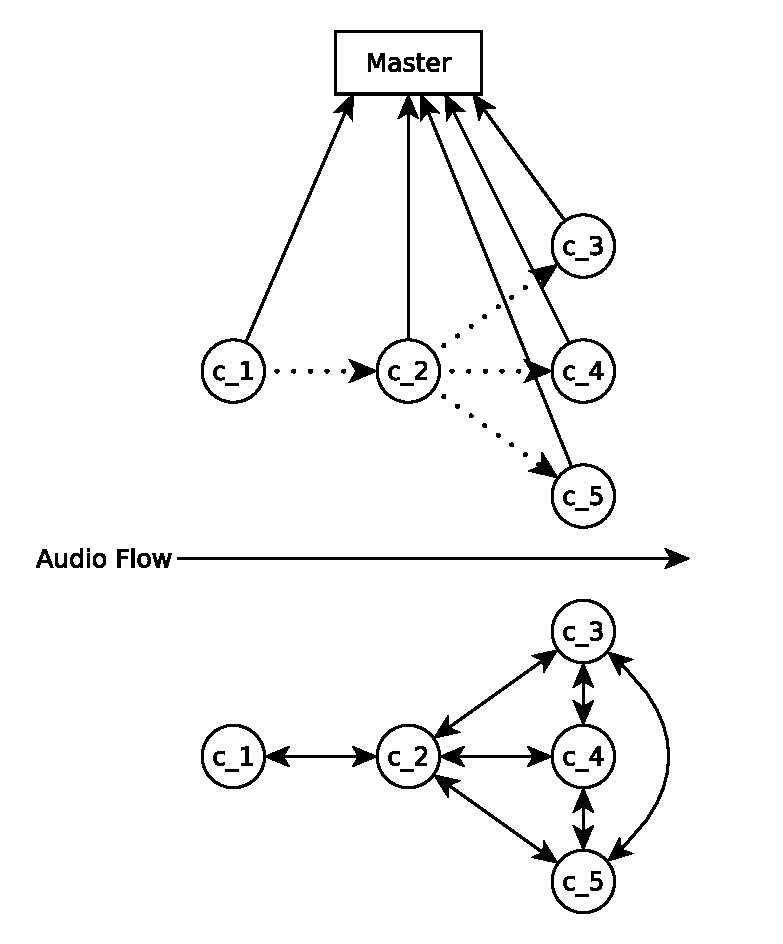
\includegraphics[width=0.66\textwidth]{diagrams/lib_central_vs_dist.pdf}
	\caption{Centralized (above) versus distributed (below) approach of determining audio formats between the components \texttt{c\_1} to \texttt{c\_5}.
		Information sending about each nodes preferred audio topic format are indicated by arrows.
		The direction of audio transmission is indicated by pointed lines above, and from left to right generally speaking.}
	\label{pic:main:lib:central_vs_dist}
\end{figure}


%------------------------------

distributed vs centralised argumentsation
centralised:
es gibt eine “master” node, die sich um a) den informations (hauptsächlich audio) flow kümmert, das umfasst auch resampling-punkte 
synchronisiert auch die daten, falls eine einzelne msg rausgeschickt wird (siehe interfaces->outside)
distributed:
jede komponente muss den info-flow einzeln berechnen, also muss er deterministisch zu berechnen sein
argumente:
bei definition von festen schnittstellen sowohl innerhalb als auch außerhalb ist centralised nicht unbedingt notwendig
centralised bietet den vorteil, dass der aufbau der pipeline nur einmal berechnet werden muss (und er damit nicht komplett deterministisch sein muss)
centralised läuft grade bei der definition fester schnittstellen die gefahr, msgs einfach nur zu relayen
momentan gäbe es zusätzlich noch die aufgabe, die jeweiligen to-from timestamp zuzuordnen (allerdings steht dafür die schnittstelle auch noch nicht, siehe )
centralised bietet einfache möglichkeiten, informationen zusammenzutragen und als bündel auszugeben, weil einfacher berechenbar ist, welche komponenten bereits ihre arbeit erledigt haben und welche noch nicht -> synchronisation
aktuell macht centralised mehr sinn

%---------------------
Argumentation for choosable audio formats
Pro:
Resampling is bad, loss of information and artifacts WILL happen
Upsampling in particular is problematic.
Some nodes may be dependent on a specific format, others won’t
eg. energy or decibel based VAD is more or less independent
Beamforming may also create audio with a specific format
To reduce information loss and artifacts, reducing the amount of resampling to a minimum is required
Audio “generating” nodes may be suited to create a wide range of formats. To take advantage of this, giving them the chance to create audio directly suited for the next component in line could make an otherwise necessary resampling step unnecessary
Con:
More complex than just using one standard format and resampling between every time
esiaf code complexity as well as node code complexity

%-------------------------

Argumentation about adaptive configuration changes
Best Case: Nodes can declare several different audio formats (if they support them, e.g. loudness/ energy based VAD) and esiaf makes use of them, i.e. chooses one of these formats according to the formats of directly connected nodes.
Problems: 
In- \& Output mapping may not be trivial
changing output format may not require to change input format
regardless, to achieve less resamples, nodes(!, not esiaf) would have to implement a callback function on changed config; this would however lead to greatly reduced usability and would counterproductive to the goal of easy and fast prototyping
Proposed solution: 
All in-\& output topics should be registered with only one format. Esiaf will then resample between nodes. Nodes which support several audio formats should be configured manually and accordingly beforehand. 
Pro:
Allowing only one format for each in-\& output reduces cost for audio flow generation and calculation of formats and resampling points tremendously
Mapping the input and output topics of each singular node -eg. beamformers- may also prove difficult for the orchestrator. Having only preconfigured formats negates this problem.
Con:
Manual configuration is expected from users, which is not exactly what is favorable

%-------------------------------
